\documentclass[a4paper,10pt]{article}
\usepackage{amsmath}
\usepackage{array}
\usepackage{graphicx}
\usepackage{url}
\usepackage[hidelinks]{hyperref}
\renewcommand{\UrlBreaks}{\do\/\do\_\do\.}

% The node's TeX installation has no geometry/booktabs/caption packages.
\setlength{\textwidth}{6.4in}
\setlength{\oddsidemargin}{-0.07in}
\setlength{\evensidemargin}{-0.07in}
\setlength{\topmargin}{-0.55in}
\setlength{\textheight}{9.6in}
\setlength{\parindent}{0pt}
\setlength{\parskip}{0.5em}
\renewcommand{\arraystretch}{1.12}
\graphicspath{{figures/}}

\newcommand{\garnet}{\texttt{GARNET}}
\newcommand{\genfoam}{GeN-Foam}
\newcommand{\code}[1]{\texttt{#1}}
\newcommand{\tablefile}[1]{\begin{center}\resizebox{\ifdim\width>\textwidth\textwidth\else\width\fi}{!}{\input{tables/#1}}\end{center}}
\newcommand{\kOneD}{0.994256}
\newcommand{\kThreeD}{0.9943}
\newcommand{\kThreeDspread}{14}
\newcommand{\kGenFoam}{0.980106}
\newcommand{\GenFoamGap}{-1417}
\newcommand{\DataGap}{-574}


\title{\textbf{Godiva with \genfoam's S$_N$ Data}\\
\large \garnet{} 1D and 3D discrete ordinates against the \genfoam{} Godiva\_SN tutorial}
\author{\garnet{} verification report}
\date{26 November 2026}

\begin{document}
\sloppy
\maketitle

\section*{Summary}

\genfoam's \code{Godiva\_SN} tutorial solves the bare HEU sphere Godiva
($R = 8.7407$~cm) with its finite-volume S$_N$ solver, 23-group data with P2
scattering, and checks $k = \kGenFoam$. Godiva is critical ($k = 1.000$). This
report replicates the case in \garnet{} with \genfoam's own nuclear data, read
in place, and explains the tutorial's value.

\begin{itemize}
\item \textbf{The data give $k = \kOneD$ when converged.} A 1D spherical S$_N$
  solution, mesh- and angle-extrapolated, is \DataGap~pcm below the experiment.
  This is a property of the 23-group data, not of either solver.
\item \textbf{3D prisms agree.} \garnet's 3D triangular-prism S$_N$ with P2
  scattering, extrapolated over five meshes (12,216 to 501,906 prisms),
  gives $k = \kThreeD \pm 0.000\kThreeDspread$. That matches the 1D value
  within the spread of the extrapolation fits.
\item \textbf{\genfoam's \kGenFoam{} is first-order discretization error}
  (\GenFoamGap~pcm).
  \begin{itemize}
  \item Its 32-direction quadrature integrates the P2 harmonics with a
    22\,\% error. Yet in \garnet's discretization it changes $k$ by only 1 to
    11~pcm.
  \item \garnet's first-order upwind (step) scheme with \genfoam's
    quadrature, on prisms of the volume of \genfoam's tetrahedra, gives
    0.977 to 0.982. That brackets \kGenFoam.
  \end{itemize}
\item \textbf{New in \garnet{} for this study:}
  \begin{itemize}
  \item the \genfoam{} \code{nuclearData} and \code{quadratureSet} readers;
  \item a 1D spherical S$_N$ solver;
  \item P$_L$ scattering and user ordinate sets on 3D prisms;
  \item a second-order (in $z$) six-corner prism discretization;
  \item a sphere-on-prisms geometry;
  \item a group-resident sweep-table cache;
  \item a lagged-factorization CMFD.
  \end{itemize}
  Every new feature has verification tests that fail on a deliberate defect.
\end{itemize}

\section{The case and its data}

The tutorial (\genfoam{} develop branch, 2025-09-30) solves the sphere on
177,655 cells, mostly tetrahedra, with one vacuum patch.
\begin{itemize}
\item \textbf{Solver:} first-order upwind finite volume; each (group,
  direction) equation is solved by BiCGStab; at most three inner iterations per
  group; power iteration through the time loop, without acceleration.
\item \textbf{Its regression check:} 20 power iterations on four cores, then
  $k = \kGenFoam$ to 0.1\,\%. That is not a converged eigenvalue.
\end{itemize}

\textbf{Data.} The data are read in place from the tutorial's
\url{constant/neutroRegion/nuclearData} by
\code{garnet.genfoam.read\_nuclear\_data}. They are
not copied into the \garnet{} repository. The conventions were taken from
\genfoam's S$_N$ source and checked independently:
\begin{itemize}
\item \code{scatteringMatrixP$l$}$[J][I]$ scatters from group $J$ to group $I$,
  without the $(2l+1)$ factor. The file's diffusion coefficients equal
  $1/(3(\Sigma_t - \sum_{g'} \Sigma_{s1,g\to g'}))$ to 0.4\,\% in groups 2--18.
  With the factor they would be 13--39\,\% off.
\item The S$_N$ collision term is \code{sigmaRemoval} plus the P0 self-scatter.
\item The equilibrium fission spectrum is $(1-\beta)\chi_p + \beta\chi_d$, with
  $\beta = 637$~pcm.
\item The file carries P0--P5 moments. The solver uses \code{legendreMoments 3},
  that is P2.
\end{itemize}

\section{One-dimensional reference}

\code{garnet.sphere\_sn} solves the 1D spherical S$_N$ equations:
\begin{itemize}
\item diamond differencing with angular redistribution;
\item Gauss--Legendre ordinates;
\item P$_L$ scattering;
\item set-to-zero fixups.
\end{itemize}
It reproduces the exactly critical LA-13511 spheres (Sood et al.\ 1999) within
1~pcm after angular extrapolation (problems 14, 24, 41, 43, 55). Figure~\ref{fig:oned}
shows the convergence for Godiva: the mesh error is second order, and the angular
error falls as $N^{-2}$.

\begin{figure}[h]
\centering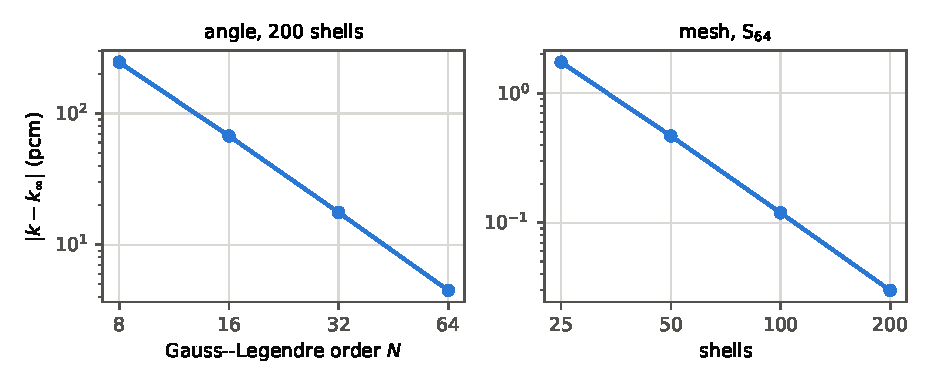
\includegraphics[width=0.85\textwidth]{oned_convergence}
\caption{1D spherical S$_N$, Godiva with \genfoam's data, P2: departure from
the extrapolated $k$ against the Gauss--Legendre order (200 shells) and the
number of equal shells (S$_{64}$).}
\label{fig:oned}
\end{figure}

\tablefile{oned}
\begin{itemize}
\item P2 is converged in scattering order: P3 and P5 differ by 3~pcm or less.
\item The anisotropy matters, because fast elastic scattering on uranium is
  strongly forward peaked ($\Sigma_{s1}/\Sigma_{s0} = 0.86$ in the first group):
  \begin{itemize}
  \item P0 with the true total cross section overestimates $k$ by 10,700~pcm;
  \item transport-corrected P0 is 330--400~pcm off.
  \end{itemize}
\end{itemize}

\section{Three-dimensional model}

\textbf{Mesh and geometry.}
\begin{itemize}
\item The sphere is meshed with \garnet's extruded triangular prisms,
  triangle side $h$ and height $h\sqrt{3}/2$.
\item \code{sphere\_on\_prisms} integrates each prism's covered volume
  exactly: closed-form triangle--disk areas, with 32-point Gauss--Legendre
  quadrature over $z$ inside each layer. It then rescales the partial prisms
  so the fuel volume is exact.
\item Partly covered prisms are fuel blended with void at their covered
  fraction.
\end{itemize}

\textbf{Discretization and solve.}
\begin{itemize}
\item \textbf{Spatial scheme:} simple corner balance (SCB) on six corners per
  prism, three in-plane corners times a lower and an upper half. The halves
  are coupled through a mid-height face that carries their average.
\item \textbf{Why six corners:} the previous three-corner prism upwinded the
  axial faces. It was first order in $z$, and on the exactly critical Sood~14
  sphere its error fell as $1/h$ ($-5192 \to -1847$~pcm from 12 to 32 cells
  across). With six corners a slab along $z$ converges at second order, and
  the sphere error drops to $-3481/-2251/-1227$~pcm at 12/16/24 cells.
\item \textbf{Scattering:} P2, with the full real spherical-harmonic basis.
  The 2D build keeps only the $z$-even half.
\item \textbf{Ordinates:} the product Gauss--Legendre $\times$ uniform
  azimuthal set $8\times16$, 128 directions, exact for the harmonics to
  $l = 4$.
\item \textbf{Outer solve:} power iteration with Anderson mixing of the
  fission source, on one GH200 with level-scheduled sweeps.
\end{itemize}

\section{Results}

\subsection{Mesh convergence}

\tablefile{mesh}

The error falls as $h^p$ with $p \approx 1.5$. The order is set by the blended
curved surface, not by the transport scheme. The verified 2D Sood~13 cylinder
on triangles, with the same blend, shows the same behaviour: $-585$~pcm at 24
cells across, $-233$~pcm at 48.

The extrapolation $k(h) = k_\infty - C h^p$ depends mildly on which meshes are
fitted:

\tablefile{fits}

The fits give $k_\infty = \kThreeD \pm 0.000\kThreeDspread$. The 1D reference
\kOneD{} lies inside that range. Figure~\ref{fig:kh} shows the sequence and
the fit.

\begin{figure}[h]
\centering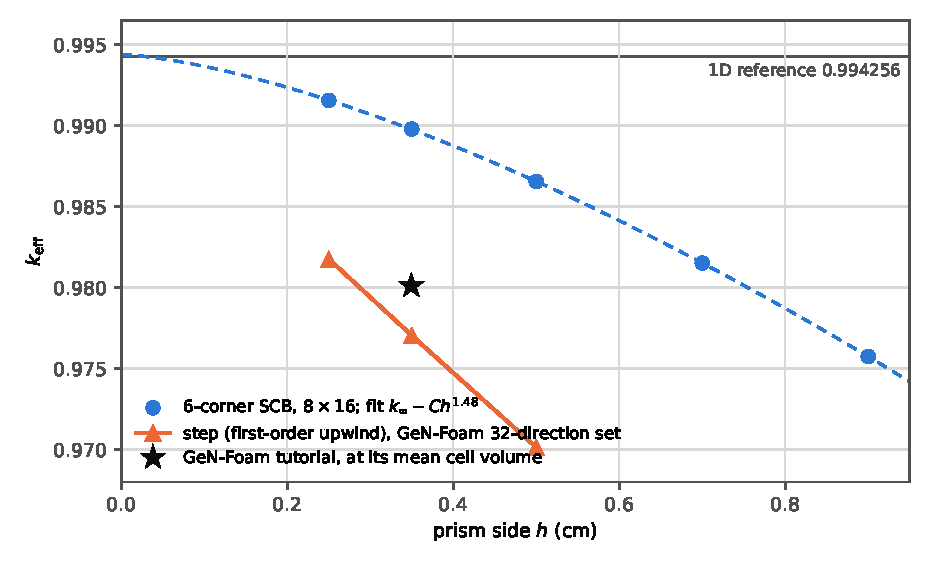
\includegraphics[width=0.85\textwidth]{k_vs_h}
\caption{Godiva on prisms, P2, \genfoam's data. Blue: six-corner SCB with the
$8\times16$ set, and the fit over all five meshes. Orange: the first-order step
scheme with \genfoam's 32-direction set. Star: \genfoam's tutorial value,
placed at the prism side whose volume equals its mean cell volume
(0.016~cm$^3$).}
\label{fig:kh}
\end{figure}

\subsection{Angular quadrature}

The other ordinate sets change $k$ by the amounts below, in pcm relative to
$8\times16$ at the same mesh. The ``P2 Gram error'' is the largest error of the
set's Gram matrix of the real harmonics up to $l = 2$.

\tablefile{quad}

\begin{itemize}
\item \textbf{$16\times32$ (512 directions)} changes $k$ by $+20$ and
  $+12$~pcm. The change shrinks with $h$, so the $8\times16$ angular error at
  $h \to 0$ is below about 10~pcm.
\item \textbf{\genfoam's sets} are not P2-exact. Its default set has a Gram
  error of $4.4\times10^{-2}$ on a diagonal of $0.2$. Even so, they change $k$
  by only $-2$ to $+11$~pcm.
\item \textbf{Why the comparison is like for like:} by the addition theorem,
  \garnet's moment form of the scattering source equals \genfoam's
  direction-pair form on any set. Running \genfoam's set in \garnet{} therefore
  uses exactly its discrete scattering operator.
\end{itemize}

\subsection{What \genfoam's \kGenFoam{} is}

\genfoam's tetrahedra have a mean volume of 0.016~cm$^3$, about that of a
\garnet{} prism with $h = 0.35$~cm. The table below gives \garnet's first-order
upwind (step) scheme with \genfoam's 32-direction set.

\tablefile{step}

\begin{itemize}
\item \textbf{The step scheme brackets \genfoam's value.} At \genfoam's
  resolution the first-order upwind error is 1250--1720~pcm, and \genfoam's
  \kGenFoam{} ($\GenFoamGap$~pcm) lies between the $h = 0.35$ and
  $h = 0.25$ results.
\item \textbf{The second-order scheme is 3--4 times closer:} the six-corner
  SCB at the same resolution is off by 450~pcm.
\item \textbf{Not separated:} tetrahedra against prisms, \genfoam's 20
  unaccelerated power iterations, and its surface representation. These are
  differences of a few hundred pcm at most.
\end{itemize}

\section{Cost and solver findings}

\begin{itemize}
\item \textbf{CMFD drift matrices factorize slowly in 3D.} At 65,610
  cells, SuperLU with COLAMD takes 28~s per group and fills
  $10^8$ nonzeros. The other orderings were no better.
  \begin{itemize}
  \item With 23 groups refactorized every outer, run time grew as $N^2$. The
    $h = 0.35$ CMFD runs did not finish in 16~h.
  \item Smoothed-aggregation AMG, AIR and ILU preconditioners all need
    150--220 GMRES iterations on these barely diagonally dominant matrices.
  \end{itemize}
\item \textbf{Lagged factorization} (\code{cmfd\_reuse}) keeps each group's
  last LU as the preconditioner of GMRES on the new matrix. At $h = 0.5$ it
  gives the same $k$ to $10^{-14}$ in 1533~s instead of 6289~s.
\item \textbf{For Godiva, power iteration is better still.}
  \begin{itemize}
  \item With Anderson mixing it converges in 12--13 outers, and $k$ equals
    the CMFD value to $7\times10^{-9}$.
  \item At $h = 0.9$ it takes 43~s instead of 202~s.
  \item Its cost is the transport sweep alone, which is linear in $N$:
    6~min at $h = 0.35$ and 15~min at $h = 0.25$.
  \end{itemize}
\item \textbf{Device-side current fold.} The CMFD current fold now runs on the
  device. A one-group sweep-table cache (\code{level\_cache="group"}) keeps
  the $6\times6$ corner inverses of only the group being swept. Without it,
  all 23 groups would need 150~GB or more at $h \le 0.35$.
\item \textbf{Open:}
  \begin{itemize}
  \item CUDA-graph replay of the level sweep fails with an illegal memory
    access at 500,000 prisms; running without graphs works.
  \item pyamg has no aarch64 wheel. It is built from source by
    \code{slurm/build\_pyamg\_gh.sh}.
  \end{itemize}
\end{itemize}

\section{Verification of the new features}

Every new test was shown to fail on a deliberate defect. All of them, with the
existing tri-S$_N$, transient, Sood and kernel suites (178 tests), pass on CPU;
the GPU paths pass on a GH200.

\begin{itemize}
\item \textbf{1D spherical S$_N$} (\code{test\_sphere\_sn.py}):
  \begin{itemize}
  \item Sood spheres critical; problem 14 flux ratios;
  \item broken without angular redistribution, without the P1 moment, or with
    a coarse quadrature.
  \end{itemize}
\item \textbf{\genfoam{} reader} (\code{test\_genfoam.py}):
  \begin{itemize}
  \item a synthetic dictionary: unit conversions, conventions, the two-group
    $k_\infty$ formula, and folding of the $\chi$ sum;
  \item the real data's D--P1 consistency;
  \item broken with a transposed matrix, or with the $(2l+1)$ factor.
  \end{itemize}
\item \textbf{3D P$_L$ and user quadrature}
  (\code{test\_tri\_sn\_3d\_anisotropic.py}):
  \begin{itemize}
  \item Sood P1/P2 slabs along $z$ critical within the S$_{64}$ floor;
  \item levels and LU engines equal to $10^{-17}$;
  \item validation of octant and \genfoam{} sets;
  \item broken with an unsigned $z$ cosine, without the moments, or without the
    angular source.
  \end{itemize}
\item \textbf{Six-corner prisms, the table cache and lagged LU}
  (\code{test\_tri\_sn\_prism\_scb.py} and
  \code{test\_gpu\_paths.py}):
  \begin{itemize}
  \item second order in $z$;
  \item a flat-in-$z$ problem identical with three or six corners;
  \item levels and LU engines equal, with both caches;
  \item lagged LU equal to refactorizing;
  \item broken with an upwinded mid-height face, a stale table cache, or a
    stale LU without the GMRES correction.
  \end{itemize}
\end{itemize}

\section{Reproduction}

All commands below run from the repository root; \code{ND} is the tutorial's
\code{nuclearData}.
\begin{itemize}
\item 1D: \code{python tools/godiva\_1d.py ND OUT}.
\item 3D, one run per mesh on a GH200 (\code{slurm/run\_garnet\_gh.sh}):
  \code{python tools/godiva\_3d.py ND h accel=power [quad=8x16|16x32|path]
  [scheme=scb|step] [graphs=0]}.
\item This report: copy the JSON records into \code{data/3d/}, then run
  \code{make PYTHON=...} in this directory.
\end{itemize}

\end{document}
